\chapter{Введение отношения порядка на множестве параметров аппроксимирующих моделей}

Рассматривается проблема введения отношения порядка на множестве параметров сложных аппроксимирующих моделей.
В качестве параметрических моделей исследуются линейные и нейросетевые модели.
Предполагается, что число параметров нейросети можно существенно снизить без значимой потери качества и значимого повышения дисперсии функции ошибки.
Предлагаются методы задания порядка на основе ковариационной матрицы градиентов функции ошибки по параметрам модели и на основе ковариационной матрицы апостериорного распределения параметров.
Показано, что полученный порядок указывает на релевантность параметров в рамках обученной нейросетевой модели: от наимеенее релевантных параметров до наиболее релевантных параметров.

Множество параметров упорядочивается по возрастанию дисперсии: от параметра с минимальной дисперсией до параметра с максимальной дисперсией градиента функции ошибки по соответствующему параметру модели. Предполагается, что малая дисперсия градиента указывает на то, что соответствующий параметр можно зафиксировать.

Для задания порядка на множестве параметров при помощи ковариационной матрицы вводится предположение о том, что фиксация параметров происходит в момент, когда все параметры модели находятся в некоторой окрестности локального минимума функции ошибки. Данное условие накладывается для корректного использования итерационного метода поиска ковариационной матрицы градиентов.

Заданный порядок на множестве параметров модели используется для фиксации тех параметров модели, которые оказываются предстоящими с точки зрения заданного порядка. Сначала фиксируются те параметры, которые имеют минимальную дисперсию градиента в окрестности локального минимума функции ошибки.

Другим подходом к определению релевантности параметров предлагается анализ ковариационной матрицы параметров модели на основе метода Белсли. Метод Белсли~\cite{neychev2016} позволяет оценить мультиколлинеарность параметров, после чего удалить наиболее коррелирующие параметры.

Для анализа свойств предложенного метода задания порядка на множестве параметров проводился вычислительный эксперимент. В качестве моделей рассматривались модели различной структурной сложности: линейные модели, нейросетевые модели. Предложенный метод задания порядка сравнивается с методом, в котором порядок задан произвольным образом.

\section{Задача упорядочивания параметров аппроксимирующих моделей}
Задана выборка:
\[
\label{ch-5:eq:st:1}
\begin{aligned}
\mathfrak{D} = \bigr\{\bigr(\textbf{x}_i, y_i\bigr)\bigr\}_{i=1}^{m}, \quad \textbf{x}_{i} \in \mathbb{X} = \mathbb{R}^{n}, \quad y_i \in \mathbb{Y},
\end{aligned}
\]
где $n$~--- размерность признакового пространства, $m$~--- число объектов в выборке. Пространство ответов $\mathbb{Y} = \mathbb{R}$ в случае задачи регрессии и  $\mathbb{Y} = \{1,\ldots, R\}$ в случае задачи классификации, где $R$~--- число классов.

Задано семейство моделей параметрических функций с наперед заданной структурой:
\[
\label{ch-5:eq:st:2}
\begin{aligned}
\mathfrak{F} &= \bigr\{f\bigr(\textbf{w}\bigr):\mathbb{X} \to \mathbb{Y} | \textbf{w} \in \mathbb{R}^{p}\bigr\}, \\ 
\mathbf{h}\bigr(\textbf{w}, \textbf{x}\bigr) &= \textbf{W}_1\bm{\sigma}\bigr(\textbf{W}_2\bm{\sigma}\bigr(\ldots\bm{\sigma}\bigr(\textbf{W}_r\textbf{x}\bigr)\ldots\bigr)\bigr),\\
f_{\text{\text{cl}}}\bigr(\textbf{w}, \textbf{x}\bigr) &= \arg \max_{j \in \bigr\{1,\ldots, R\bigr\}} \text{softmax}\bigr(\mathbf{h}\bigr(\textbf{w}, \textbf{x}\bigr)\bigr)_{j}, \\ 
f_{\text{reg}}\bigr(\textbf{w}, \textbf{x}\bigr) & = \mathbf{h}\bigr(\textbf{w}, \textbf{x}\bigr), 
\end{aligned}
\]
где $p$~--- размерность пространства параметров, $r$~--- число слоев нейросети, $\textbf{w} = \text{vec}[\textbf{W}_1, \textbf{W}_2, \ldots, \textbf{W}_r]$, а $\bm{\sigma}$~--- функция активации. В случае задачи регрессии структура модели имеет вид $f_{\text{\text{reg}}}$, а в случае классификации имеет вид $f_{\text{\text{cl}}}$.
%В качестве $\tau$ рассматривается $\tau\bigr(\textbf{x}\bigr) = \textbf{x}$ в случае задачи регрессии, в случае задачи многоклассовой классификации $\bm{\sigma}\bigr(\textbf{x}\bigr) = \text{softmax}\bigr(\textbf{x}\bigr)$.
Задана функция потерь:
\[
\label{ch-5:eq:st:3}
\begin{aligned}
\mathcal{L}\bigr(\textbf{w}, \mathfrak{D}\bigr) &= \frac{1}{m}\sum_{i=1}^{m}l\bigr(\textbf{x}_{i}, y_i, \textbf{w}\bigr),\\
l_{\text{\text{reg}}}\bigr(\textbf{x}, y, \textbf{w}\bigr) &= \bigr(y - f\bigr(\textbf{w}, \textbf{x}\bigr)\bigr)^{2},\\
l_{\text{\text{cl}}}\bigr(\textbf{x}, y, \textbf{w}\bigr) &= -\sum_{j=1}^{R}\bigr([y = j]\ln\text{softmax}_j\bigr(\mathbf{h}\bigr(\textbf{w}, \textbf{x}\bigr)\bigr)\bigr),
\end{aligned}
\]
где $l_{\text{\text{reg}}}$~--- это функция ошибки на одном элементе для задачи регрессии, $l_{\text{\text{cl}}}$~--- для задачи классификации.
Оптимальный вектор параметров $\hat{\textbf{w}}$ получим минимизацией функции потерь:
\[
\label{ch-5:eq:st:0:1}
\begin{aligned}
\hat{\textbf{w}} = \arg \min_{\textbf{w}\in\mathbb{R}^{p}} \mathcal{L}\bigr(\textbf{w}, \mathfrak{D}\bigr).
\end{aligned}
\]

Для поиска оптимальных параметров модели используется градиентный метод оптимизации:
\[
\label{ch-5:eq:st:4}
\begin{aligned}
\textbf{w}_{t} = \textbf{w}_{t-1} + \Delta\textbf{w}\bigr(\textbf{g}_{S,t}, \textbf{w}_{t-1}, \textbf{w}_{t-2}, \ldots\bigr), \quad \textbf{g}_{S,t}=\frac{\partial \mathcal{L}\bigr(\textbf{w}_{t}, \textbf{X}_{S}, \textbf{Y}_{S}\bigr)}{\partial \textbf{w}},
\end{aligned}
\]
где $t$~--- номер итерации, $\textbf{g}_{S,t}$~--- значение градиента на подвыборке размера $S$, $\Delta\textbf{w}$~--- приращение вектора параметров.
 
 
Порядок на множестве параметров модели задается при помощи ковариационной матрицы $\textbf{C}$ градиентов функции ошибки $\mathcal{L}$ по параметрам модели $\textbf{w}$. Для вычисления ковариационной матрицы $\textbf{C}$ используется итерационная формула~\cite{Chunyan2016}, которая вычисляется на каждой итерации \eqref{ch-5:eq:st:4} градиентного метода оптимизации параметров:
\[
\label{ch-5:eq:st:5}
\begin{aligned}
\textbf{C}_t = \bigr(1-\kappa_t\bigr)\textbf{C}_{t-1}+\kappa_t\bigr(\textbf{g}_{1,t}-\textbf{g}_{S,t}\bigr)\bigr(\textbf{g}_{1,t}-\textbf{g}_{S,t}\bigr)^{\mathsf{T}},
\end{aligned}
\]
 где $t$~--- номер итерации, $\textbf{g}_{S,t}$~--- значение градиента на подвыборке размера $S$, $\textbf{g}_{1,t}$~--- значение градиента на первом элементе подвыборки, $\kappa_t=\frac{1}{t}$~--- параметр сглаживания, $\textbf{C}_0$ инициализируются из равномерного распределения.
 
Пусть известно $t_0$~--- число итераций, после которого все параметры находятся в некоторой локальной окрестности минимума, тогда, как показано в работе~\cite{Chunyan2016}, матрица $\textbf{C}_{t_0}$ аппроксимирует истинную ковариационную матрицу $\textbf{C}$. Ковариационная матрица $\textbf{C}_{t_0}$ используется для упорядочения параметров модели $\textbf{w}_{t_0}$. 
 
Пусть $\mathcal{I}$~---  упорядоченный вектор индексов $[1, 2, \ldots, p]$. Обозначим $\mathcal{I}_{\textbf{w}_{t_0}}$ вектор индексов, порядок которого задан при помощи ковариационной матрицы $\textbf{C}_{t_0}$. 
 
Например, если ковариационная матрица $\textbf{C}_{t_0}$  имеет вид
 $$
\begin{bmatrix}
0{,}3& 0 & 0\\
0& 0{,}2 & 0\\
0& 0 & 0{,}25\\
\end{bmatrix},
 $$
 то вектор индексов $\mathcal{I}_{\textbf{w}_{t_0}} = [3,1,2]$.
 
\paragraph{Фиксация параметров модели в процессе обучения.}
Для фиксации параметров $\textbf{w}_{t_0}$ при помощи вектора индексов $\mathcal{I}_{\textbf{w}_{t_0}}$ используется бинарный вектор $\bm{\alpha}\bigr(\zeta\bigr)$:
\[
\label{ch-5:eq:st:6}
\begin{aligned}
\alpha_i\bigr(\zeta\bigr) = \begin{cases}
   1, &\text{если }\mathcal{I}_{\textbf{w}_{t_0}}[j] \leq \zeta;\\
   0 &\text{иначе},
 \end{cases}
\end{aligned}
\]
 где $\zeta$~--- число фиксирующих параметров.
 
 Учитывая \eqref{ch-5:eq:st:6}, уравнение \eqref{ch-5:eq:st:4} приводится к виду
 \[
\label{ch-5:eq:st:7}
\begin{aligned}
\textbf{w}_{t} = \textbf{w}_{t-1} + \bm{\alpha}\bigr(\zeta\bigr)\cdot\Delta\textbf{w}\bigr(\textbf{g}_{S,t}, \textbf{w}_{t-1}, \textbf{w}_{t-2}, \ldots\bigr),
\end{aligned}
\]
где $t$~--- номер итерации, $\textbf{g}_{S,t}$~--- значение градиента на подвыборке размера $S$, $\Delta\textbf{w}$~--- приращение вектора параметров. После умножения на бинарный вектор $\bm\alpha$ часть параметров не оптимизируется, что приводит к фиксации параметров.

\section{Определение релеватности на основе метода Белсли}
Предлагается метод основанный на модификации метода Белсли. Пусть $\textbf{w}$~--- вектор параметров доставляющий минимум функционалу потерь $\mathcal{L}$ на  множестве $\mathbb{W_\mathcal{A}}$, а $\textbf{A}_\text{ps}$ соответствующая ему ковариационная матрица.

Выполним сингулярное разложение матрицы
\[
\textbf{A}_\text{ps} = \textbf{U}{\bf\Lambda}\textbf{V}^\mathsf{T}.
\]
Индекс обусловленности $\eta_{j}$ определим как отношение максимального элемента к $j$-му элементу матрицы ${\bf\Lambda}$. Для нахождения мультиколлинеарных признаков требуется найти индекс $\xi$ вида:
\[
\xi = \arg\max_{j\in \mathcal{A}}{\eta_j}.
\]

\begin{figure}[h!t]\center
\subfloat[Матрица ковариации]{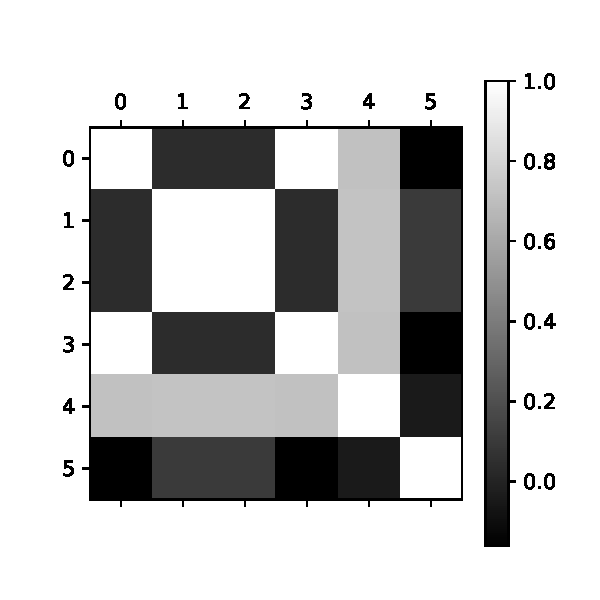
\includegraphics[width=0.5\textwidth]{results/relevant/Cov.pdf}}
\subfloat[Дисперсионные доли]{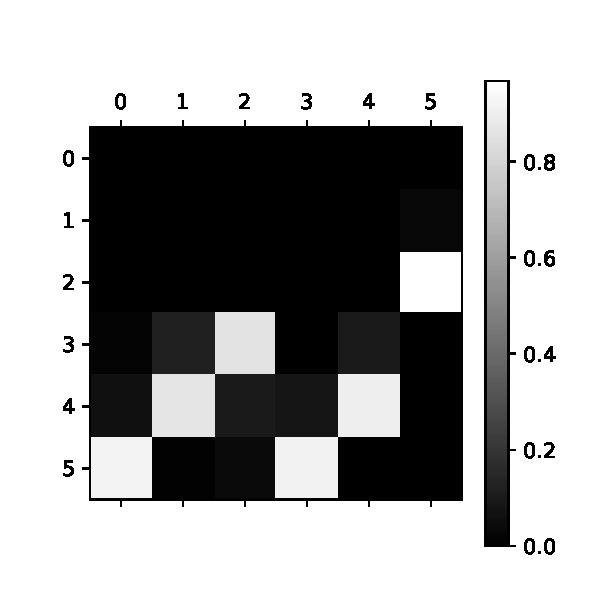
\includegraphics[width=0.5\textwidth]{results/relevant/BelslyImage.pdf}}
\caption{Илюстрация метода Белсли для анализа мультиколлинеарности параметров}
\label{CovBel}
\end{figure}

\begin{table}[h]
\begin{center}
\caption{Илюстрация метода Белсли для анализа мультиколлинеарности параметров}
\begin{tabular}{|c|cccccc|}
\hline
$\eta$ & $q_1$& $q_2$& $q_3$& $q_4$& $q_5$& $q_6$\\
\hline
$1.0$ &  $2\cdot 10^{-17}$ &  $4\cdot 10^{-17}$ &  $1\cdot 10^{-16}$ &  $2\cdot 10^{-17}$ &  $6\cdot 10^{-17}$&  $3\cdot 10^{-4}$ \\
\hline
$1.5$ &  $5\cdot 10^{-17}$ &  $9\cdot 10^{-17}$ &  $2\cdot 10^{-16}$ &  $5\cdot 10^{-17}$ &  $3\cdot 10^{-20}$ &  $3\cdot 10^{-2}$ \\
\hline
$3.3$ &  $9\cdot 10^{-18}$ &  $1\cdot 10^{-17}$ &  $2\cdot 10^{-17}$ &  $9\cdot 10^{-18}$ &  $2\cdot 10^{-19}$ &  $9\cdot 10^{-1}$ \\
\hline
$2\cdot 10^{15}$ &  $1\cdot 10^{-2}$ &  $1\cdot 10^{-1}$ &  $8\cdot 10^{-1}$ &  $2\cdot 10^{-3}$ &  $9\cdot 10^{-2}$ &  $1\cdot 10^{17}$ \\ 
\hline
$8\cdot 10^{15}$ &  $6\cdot 10^{-2}$ &  $8\cdot 10^{-1}$ &  $9\cdot 10^{-2}$ &  $8\cdot 10^{-2}$ &  $9\cdot 10^{-1}$ & $ 2\cdot 10^{17} $\\
\hline
$1\cdot 10^{16}$ &  $\bf9\cdot 10^{-1}$ &  $1\cdot 10^{-2}$& $ 4\cdot 10^{-2}$&  $\bf9\cdot 10^{-1}$ &  $1\cdot 10^{-3}$ & $ 5\cdot 10^{-21}$ \\
\hline
\end{tabular}
\label{CovBelTable}
\end{center}
\end{table}

Дисперсионный долевой коэффициент $q_{ij}$ определим как вклад $j$-го признака в дисперсию $i$-го элемента вектора параметра $\textbf{w}$:

\[
q_{ij} = \frac{u^2_{ij}/\lambda_{jj}}{\sum^n_{j=1}{u^2_{ij}/\lambda_{jj}}}.
\]

Большие значение дисперсионных долей указывают на наличие зависимости между параметрами. Находим долевые коэффициенты, которые вносят максимальный вклад в дисперсию параметра $w_\xi$:

\[
\zeta = \arg\max_{j\in \mathcal{A}}{q_{\xi j}}.
\]
Параметр с индексом $\zeta$ определим как наименее релевантный параметр нейросети. 
%Для удаления нескольких зависимых параметров за раз, предлагается удалить параметры с номерами $p \in \mathcal{A}: q_{\xi i} > \lambda  \in  \mathbb{R}_+$.

Проиллюстрируем принцип работы метода Белсли на примере. Гипотеза порождения данных: 
\[
\textbf{w} = \begin{bmatrix}
\text{sin}(x)\\
\text{cos}(x)\\
\text{2+cos}(x)\\
\text{2+sin}(x)\\
\text{cos}(x) + \text{sin}(x)\\
x
\end{bmatrix}
\]
с матрицей ковариации на рис. \ref{CovBel}.a, где $x \in [0.0, 0.02, ..., 20.0]$.


В табл. \ref{CovBelTable} приведены индексы обусловленности и соответствующие им дисперсионные доли, которые также изображены на рис. \ref{CovBel}.b. Согласно этим данным, максимальный индекс обусловленности $\eta_6 = 1.2\cdot 10^{16}$. Ему соответствуют максимальные дисперсионные доли признаков с индексами 1 и 4, которые, как видно из построения выборки, являются линейно зависимые.

\section{Анализ разных подходов к определению релевантности}
Для анализа свойств предложенного алгоритма и сравнения его с существующими проведен вычислительный эксперимент в котором параметры нейросети удалялись методами, которые описаны в разделах 3.1---3.3 и методом Белсли.

В качестве данных использовались три выборки. Выборки Wine~\cite{Wine} и Boston Housing~\cite{Boston} ~--- это реальные данные. Синтетические данные сгенерированы таким образом чтобы параметры сети мультиколинеарными. Генерация данных состояла из двух этапов. 
На первом этапе генерировался вектор параметров $\mathbf{w}_{\text{synthetic}}$:
\[
\mathbf{w}_{\text{synthetic}}  \sim \mathcal{N}(\textbf{m}_{\text{synthetic}}, \textbf{A}_{\text{synthetic}}),
\]
где 
$\textbf{m}_{\text{synthetic}} = \begin{bmatrix}
1.0\\
0.0025\\
\ldots\\
0.0025
\end{bmatrix}$,
$\textbf{A}_{\text{synthetic}} = \begin{bmatrix}
1.0& 10^{-3}& \ldots& 10^{-3}& 10^{-3}\\
10^{-3}& 1.0& \ldots& 0.95& 0.95\\
\ldots&\ldots&\ldots&\ldots&\ldots\\
10^{-3}& 0.95& \ldots& 0.95& 1.0
\end{bmatrix}$.

На втором этапе генерировалась выборка $\mathfrak{D}_{\text{synthetic}}$:
\[
\mathfrak{D}_{\text{synthetic}} = \{(\textbf{x}_i,y_i)| \textbf{x}_i \sim  \mathcal{N}(\textbf{1}, \textbf{I}), y_i = x_{i0}, i = 1 \ldots 10000\}.
\]
В приведенном выше векторе параметров $\mathbf{w}_{\text{synthetic}}$ для выборки $\mathfrak{D}_{\text{synthetic}}$, наиболее релевантным является первый параметр, а все остальные параметры являются нерелевантными. Матрица ковариации выбрана таким образом, чтобы все нерелевантные параметры являлись зависимыми величинами, что приводит к максимальной эффективности метода Белсли.

\begin{table}[h]

\begin{center}
\caption{Описание выборок для анализа метода задания порядка методом Белсли}
\begin{tabular}{|c|c|c|c|}
\hline
	Выборка &Тип задачи& Размер выборки& Число признаков\\
	\hline
	
	\multicolumn{1}{|l|}{Wine}
	&
	\multicolumn{1}{|l|}{класификация}
	 & 178 & 13\\
	\hline
	
	\multicolumn{1}{|l|}{Boston Housing}
	&
	\multicolumn{1}{|l|}{регресия}
	& 506 & 13\\
	\hline
	
	\multicolumn{1}{|l|}{Synthetic data}
	&
	\multicolumn{1}{|l|}{регресия}
	& 10000 & 100\\
\hline

\end{tabular}
\end{center}
\end{table}



Для алгоритмов тренировочная и тестовая выборки составили $80\%$ и $20\%$ соответсвенно. Критерием качества прореживания служит процент параметров нейросети, удаление которого не влечет значимой потери качества прогноза. Также критерием качества служит устойчивость нейросети к зашумленности данных. 

Качеством прогноза $R_{\text{cl}}$ модели для задачи классификации является точность прогноза модели:
\[
R_{\text{cl}} = \frac{\sum_{(\textbf{x},y)\in \mathfrak{D}} [f(\textbf{x}, \textbf{w}) = y]}{\left|\mathfrak{D}\right|},
\]

Качеством прогноза $R_{\text{rg}} $ модели для задачи регрессии является среднеквадратическое отклонение результата модели от точного:

\[
R_{\text{rg}} = \frac{\sum_{(\textbf{x},y)\in \mathfrak{D}} \left(f(\textbf{x}, \textbf{w}) - y\right)^2}{\left|\mathfrak{D}\right|},
\]

\paragraph{Wine.} Рассмотрим нейроную сеть с 13 нейронами на входе, 13 нейронами в скрытом слое и 3 нейронами на выходе.

\begin{figure}[h!t]\center
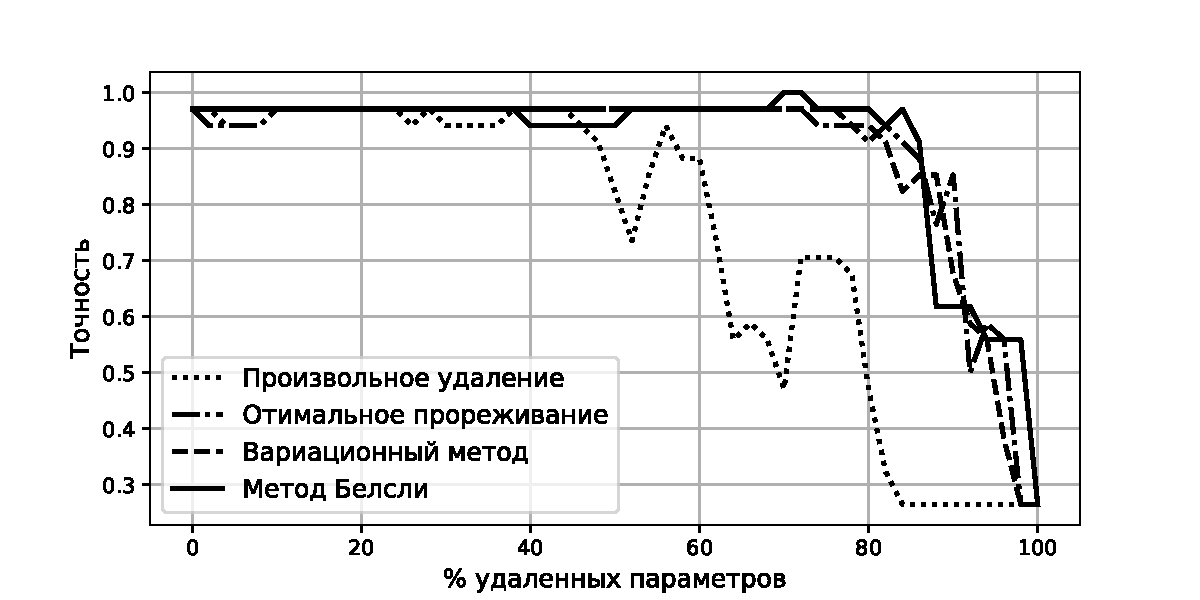
\includegraphics[width=0.8\textwidth]{results/relevant/Wine/All.pdf}\\
\caption{Качество прогноза при удаление параметров на выборке Wine}
\label{WineAll}
\end{figure}

\begin{figure}[h!t]\center
\subfloat[Произвольное удаление параметров]{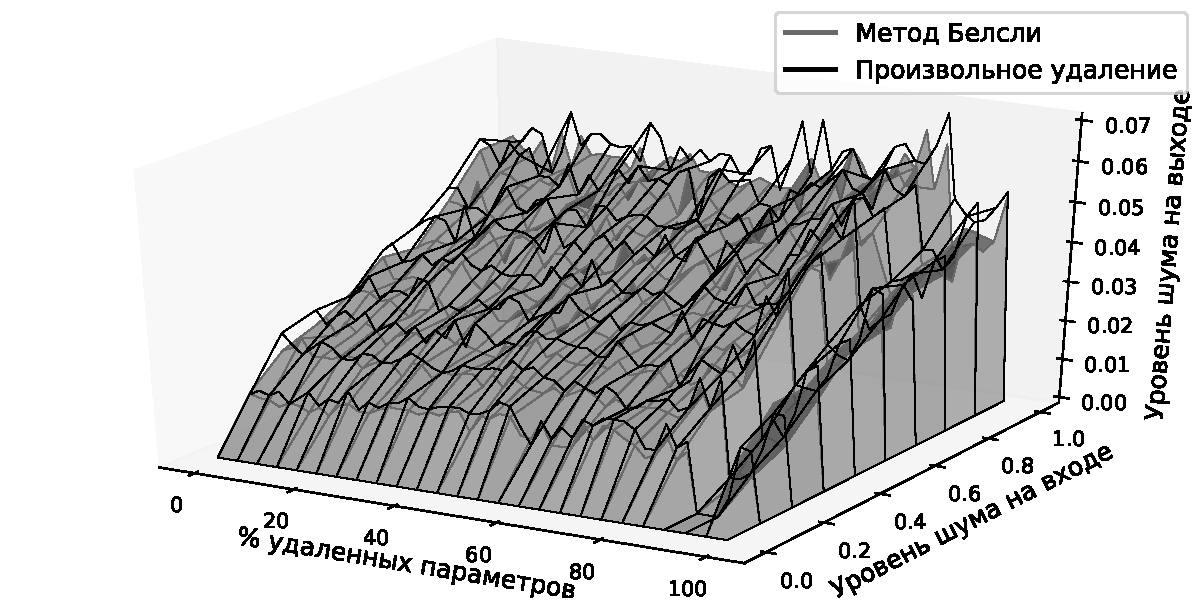
\includegraphics[width=0.5\textwidth]{results/relevant/Wine/RandomNoise3D.pdf}}
\subfloat[Оптимальное прореживание]{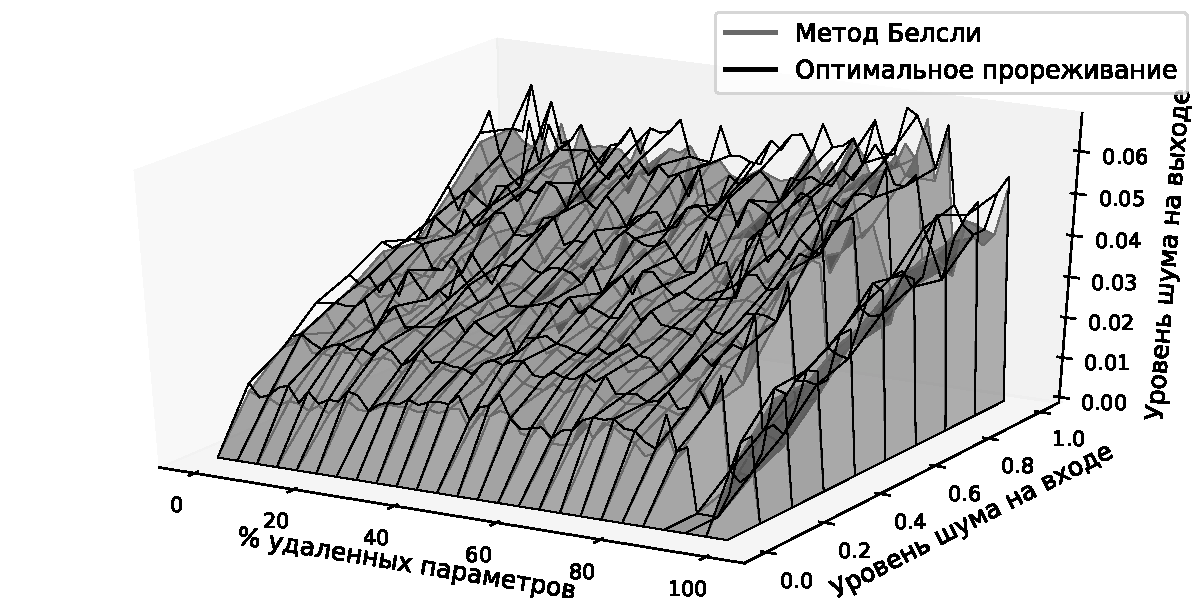
\includegraphics[width=0.5\textwidth]{results/relevant/Wine/OBDNoise3D.pdf}}\\
\subfloat[Вариационный метод]{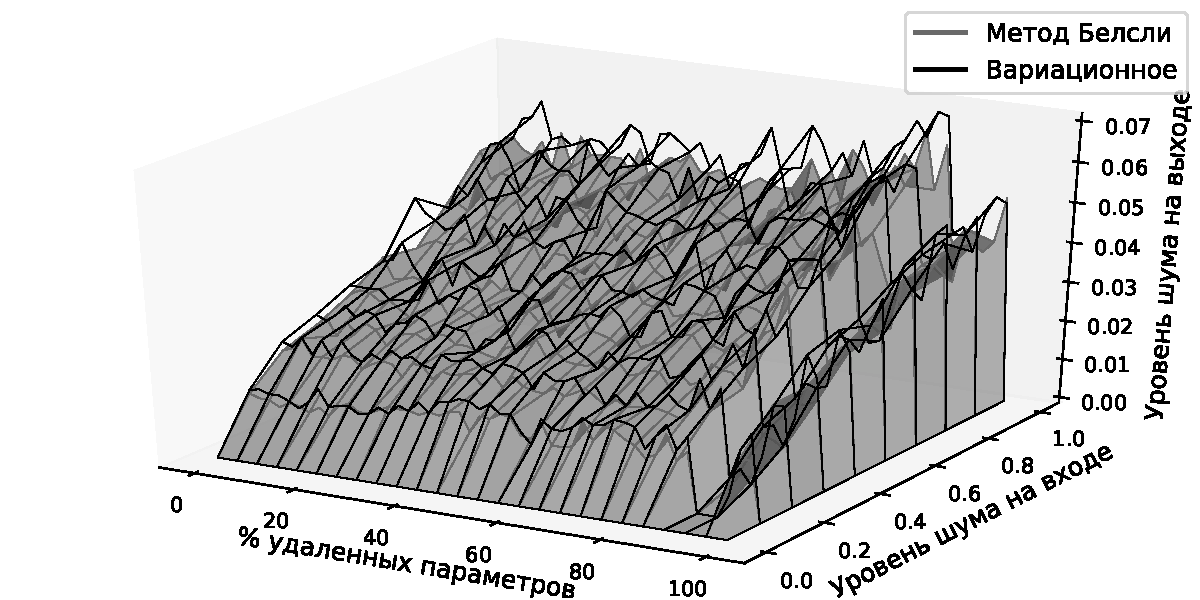
\includegraphics[width=0.5\textwidth]{results/relevant/Wine/VariationalNoise3D.pdf}}
\caption{Влияние шума в начальных данных на шум выхода нейросети на выборке Wine}
\label{WineNoise}
\end{figure}

На рис. \ref{WineAll} показано как меняется точность прогноза $R_{\text{cl}}$ при удалении параметров указанными методами. Из графика видно, что метод оптимального прореживания, вариационный метод и метод Белсли позволяют удалить $\approx80\%$ параметров и качество всех этих методов падает при удалении $\approx90\%$ параметров нейросети. 

На рис. \ref{WineNoise} показаны поверхности изменения уровня шума ответов нейросети при изменении процента удаленных параметров и уровня шума входных данных для разных методов прореживания. На графиках показано, что при удалении параметров нейросети методом Белсли шум меньше, чем при удалении параметров другими методами, на это указывает то что поверхность которая соответствует методу Белсли ниже других поверхностей.

\paragraph{Boston Housing.} Рассмотрим нейроную сеть с 13 нейронами на входе, 39 нейронами в скрытом слое и одним нейроном на выходе.

\begin{figure}[h!t]\center
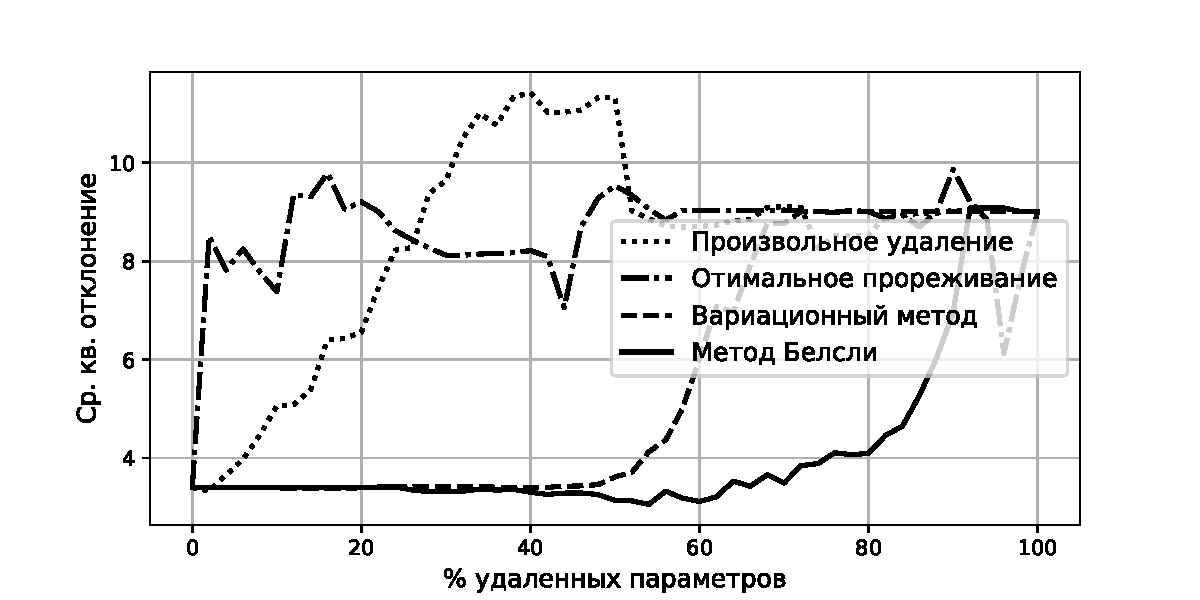
\includegraphics[width=0.8\textwidth]{results/relevant/Boston/All.pdf}\\
\caption{Качество прогноза при удаление параметров на выборке Boston}
\label{BostonAll}
\end{figure}

\begin{figure}[h!t]\center
\subfloat[Произвольное удаление параметров]{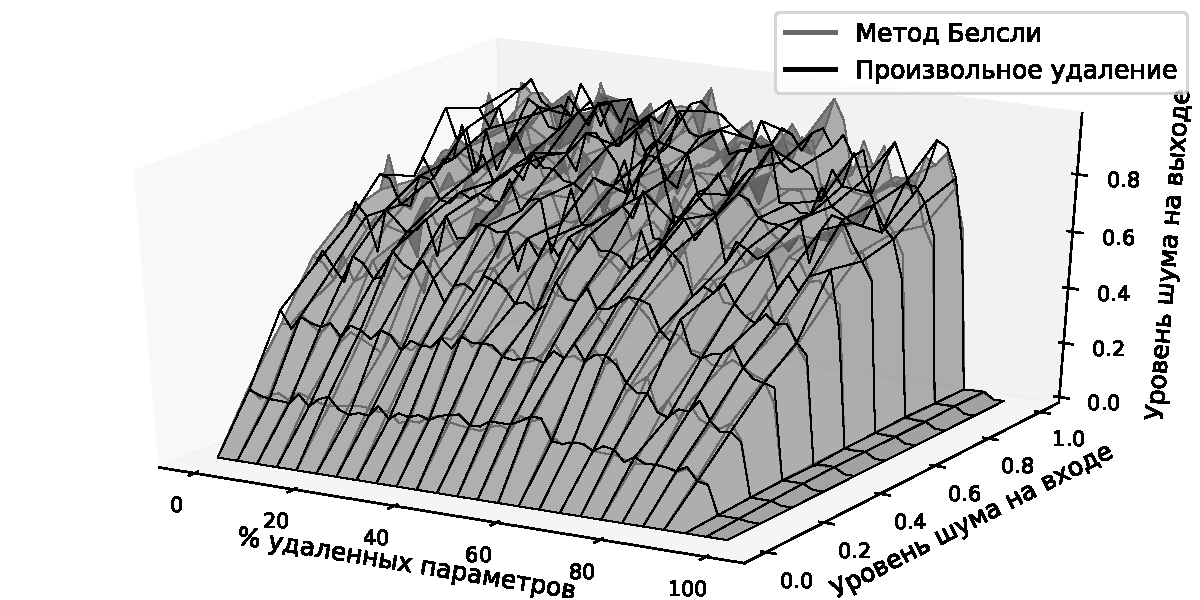
\includegraphics[width=0.5\textwidth]{results/relevant/Boston/RandomNoise3D.pdf}}
\subfloat[Оптимальное прореживание]{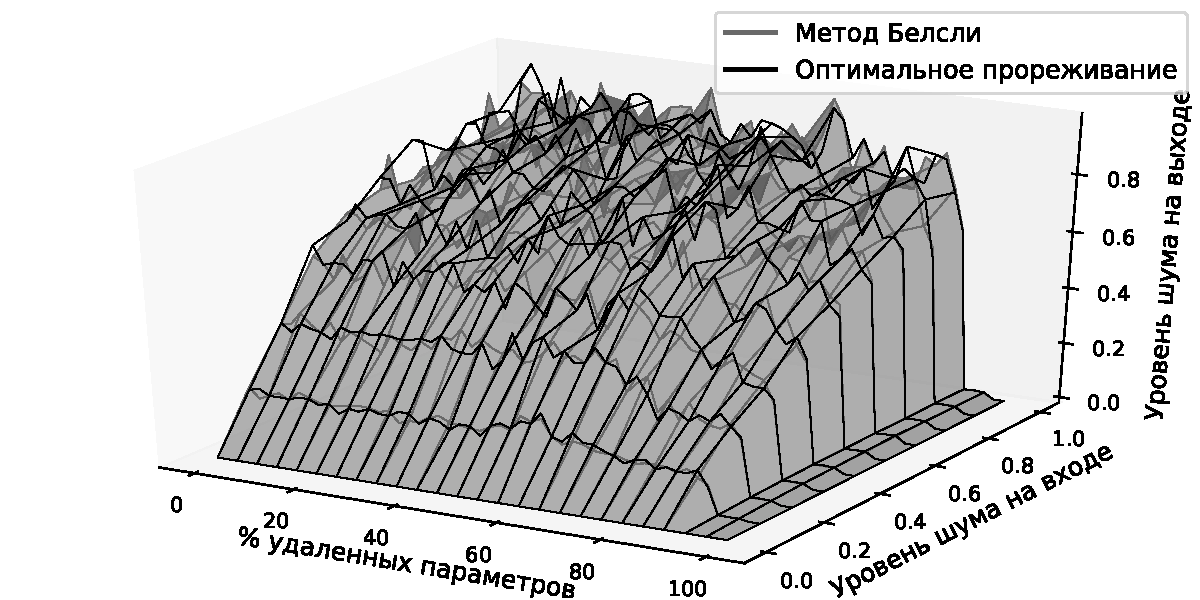
\includegraphics[width=0.5\textwidth]{results/relevant/Boston/OBDNoise3D.pdf}}\\
\subfloat[Вариационный метод]{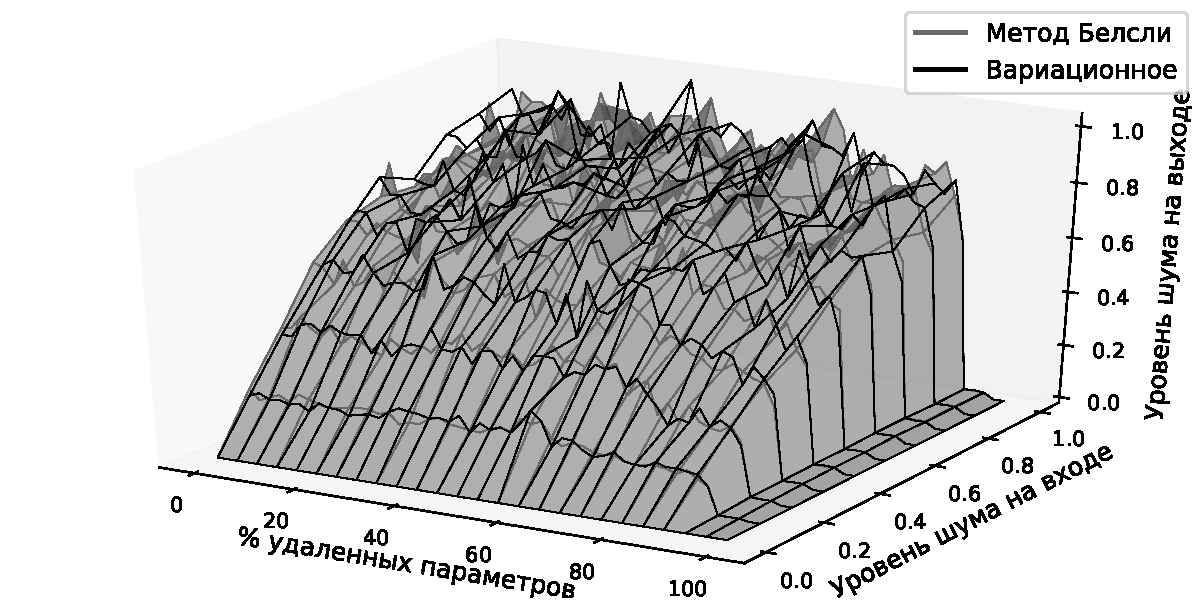
\includegraphics[width=0.5\textwidth]{results/relevant/Boston/VariationalNoise3D.pdf}}
\caption{Влияние шума в начальных данных на шум выхода нейросети на выборке Boston}
\label{BostonNoise}
\end{figure}

На рис. \ref{BostonAll} показано как меняется среднеквадратическое отклонение прогноза $\mathsf{R}_{\text{rg}}$ от точного ответа  при удалении параметров указанными методами. График показывает, что метод Белсли является более эффективным, чем другие методы, так как позволяет удалить больше параметров нейросети без потери качества.

На рис. \ref{BostonNoise} показаны поверхности изменения уровня шума ответов нейросети при изменении процента удаленных параметров и уровня шума входных данных для разных методов прореживания. График показывает, что уровень шума всех методов одинаковый, так как поверхности всех методов находятся на одном уровне.


\paragraph{Синтетические данные.} Рассмотрим нейроную сеть с 100 нейронами на входе и одним нейроном на выходе.

\begin{figure}[h!t]\center
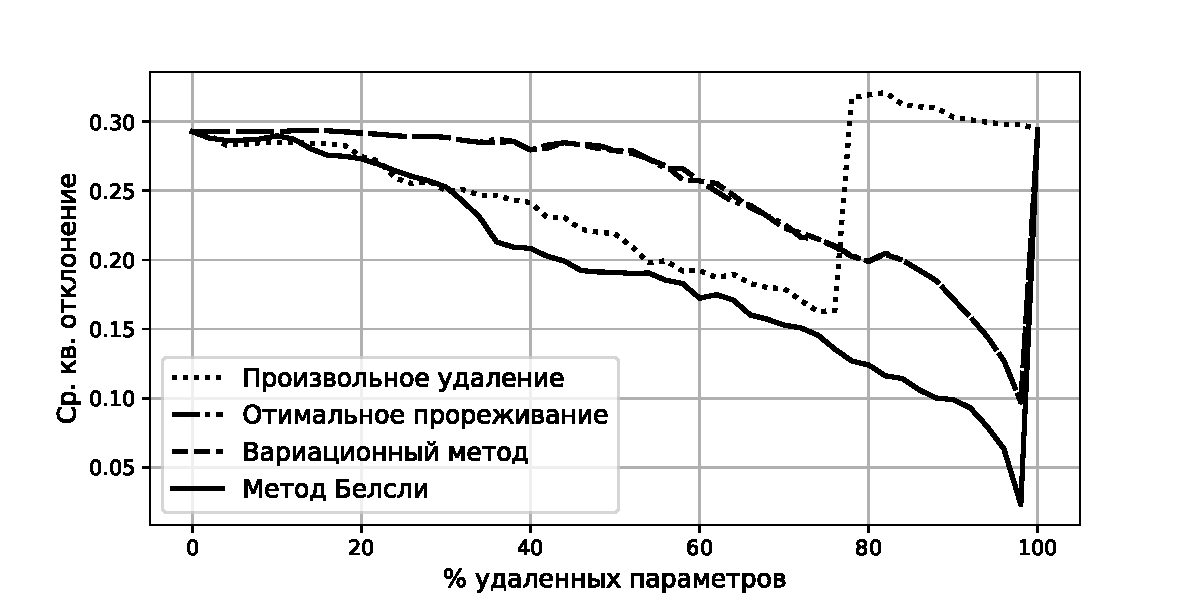
\includegraphics[width=0.8\textwidth]{results/relevant/Data1/All.pdf}\\
\caption{Качество прогноза при удаление параметров на синтетической выборке}
\label{Data1All}
\end{figure}

\begin{figure}[h!t]\center
\subfloat[Произвольное удаление параметров]{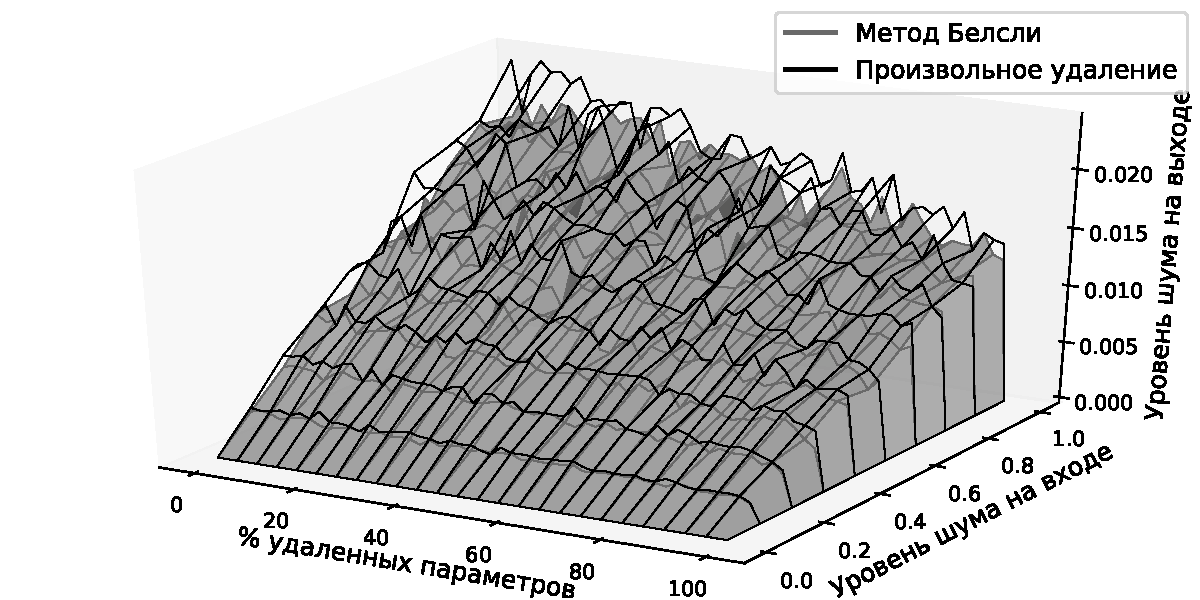
\includegraphics[width=0.5\textwidth]{results/relevant/Data1/RandomNoise3D.pdf}}
\subfloat[Оптимальное прореживание]{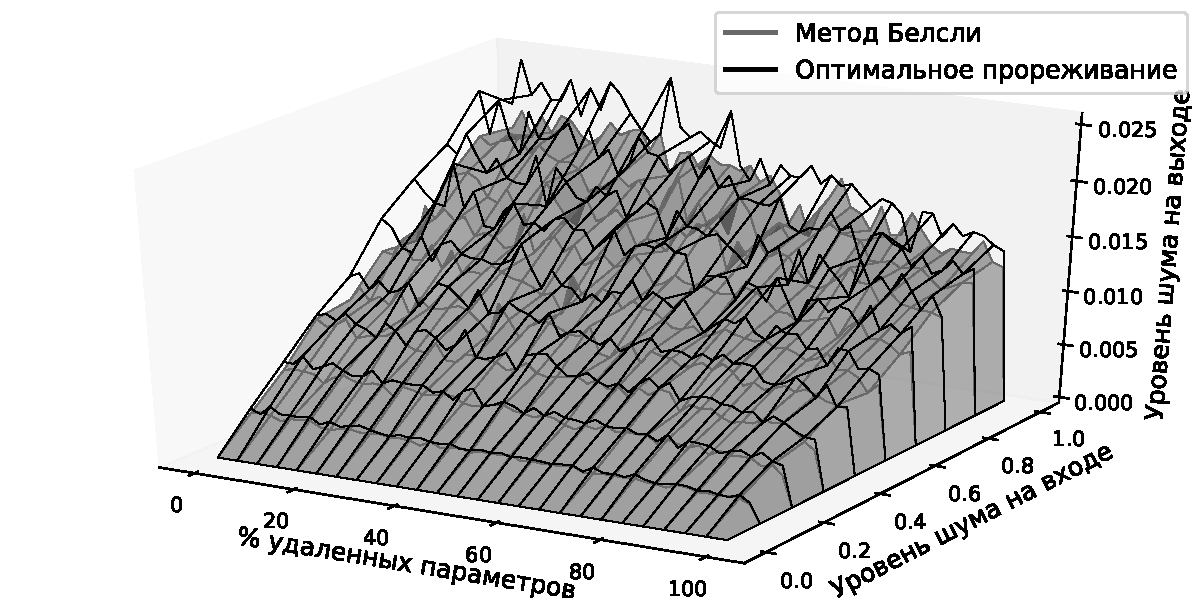
\includegraphics[width=0.5\textwidth]{results/relevant/Data1/OBDNoise3D.pdf}}\\
\subfloat[Вариационный метод]{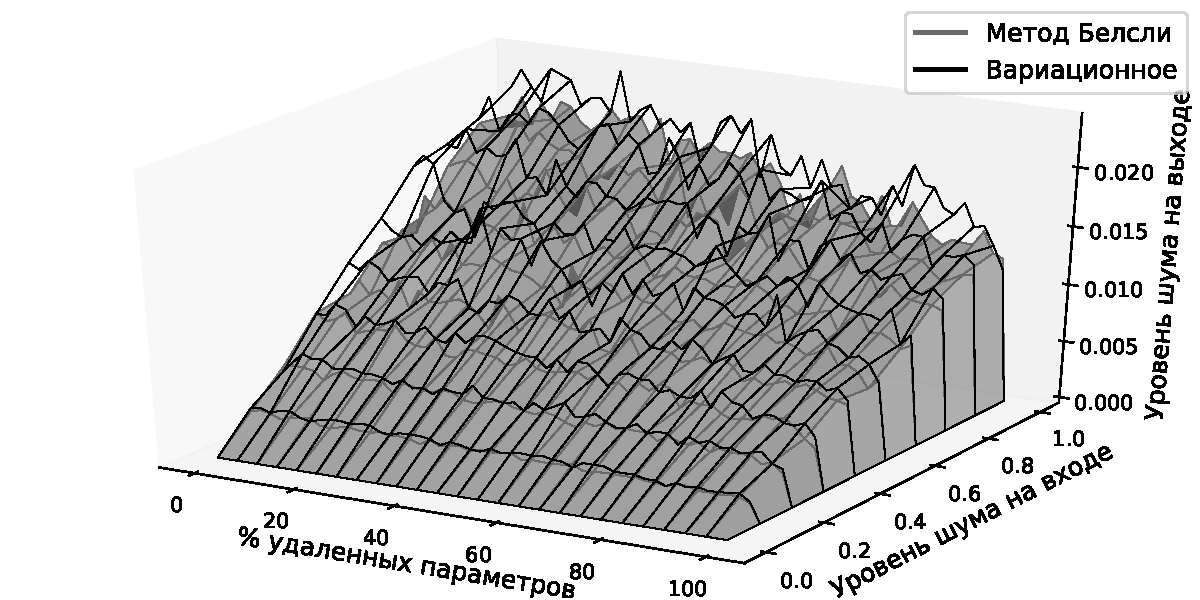
\includegraphics[width=0.5\textwidth]{results/relevant/Data1/VariationalNoise3D.pdf}}
\caption{Влияние шума в начальных данных на шум выхода нейросети на синтетической выборке}
\label{Data1Noise}
\end{figure}

На рис. \ref{Data1All} показано как меняется среднеквадратическое отклонение прогноза от $\mathsf{R}_{\text{rg}}$ точного ответа при удалении параметров указанными методами. График показывает, что удаление параметров методом Белсли являеться более эффективным чем другие методы прореживания, так как качество прогноза нейросети повышается при удалении шумовых параметров.

На рис. \ref{Data1Noise} показаны поверхности изменения уровня шума ответов нейросети при изменении процента удаленных параметров и уровня шума входных данных для разных методов прореживания. На графиках показано, что при удалении параметров нейросети методом Белсли шум меньше, чем при удалении параметров другими методами, так как поверхность которая соответствует методу Белсли ниже других поверхностей.


\section{Вычислительный эксперимент по упорядочиванию параметров}

\begin{table}[h!t]
\begin{center}
\caption{Описание выборок, используемых в эксперименте по анализу метода задания порядка на основе анализа ковариационной матрицы градиентов}
\label{ch-5:tb:ex:1}
\begin{tabular}{|c|c|c|c|c|c|}
\hline
	Выборка, $\mathfrak{D}$& Тип & Число& Модель& Число \\
	&& признаков, $n$&&параметров, $p$\\
	\hline
	\multicolumn{1}{|l|}{Boston Housing}&
	Регрессия& 13& Нейросеть& 301\\
	\hline
	\multicolumn{1}{|l|}{MNIST}&
	Классификация& 784& Нейросеть& 7960\\
	\hline
	\multicolumn{1}{|l|}{Synthetic 3}&
	Регрессия& 200& Линейная& 200\\
	\hline
	\multicolumn{1}{|l|}{Synthetic 2}&
	Классификация& 200& Линейная& 200\\
	\hline
	\multicolumn{1}{|l|}{Synthetic 1}&
	Регрессия& 200& Нейросеть& 4041\\
\hline

\end{tabular}
\end{center}
\end{table}

Для анализа результатов, полученных предложенным алгоритмом, проводится вычислительный эксперимент. В качестве данных используются синтетические и реальные данные, которые описаны в табл. \ref{ch-5:tb:ex:1}. Выборки MNIST~\cite{mnist} и Boston Housing~\cite{Boston} рассматриваются в качестве реальных данных, для которых решается задача классификации и регрессии соответственно. Алгоритм генерации синтетической выборки:
\[
\label{eq:ex:1}
\begin{aligned}
\mathfrak{D}_{\text{\text{reg}}} &= \bigr\{\bigr(\textbf{x}_i, y_i \bigr) |\textbf{x}_{i}\sim\mathcal{N}\bigr(\textbf{0}, \textbf{I}_{n}\bigr), y_{i}\sim\mathcal{N}\bigr(\textbf{w}^{\mathsf{T}}\textbf{x}_{i}, \textbf{I}_{n}\bigr),  \textbf{w} \sim \mathcal{N}\bigr(\textbf{0}, \textbf{I}_{n}\bigr)\bigr\},\\
\mathfrak{D}_{\text{\text{cl}}} &= \bigr\{\bigr(\textbf{x}_i, y_i \bigr) |\textbf{x}_{i}\sim\mathcal{N}\bigr(\textbf{0}, \textbf{I}_{n}\bigr), y_{i}\sim\mathcal{B}e\bigr(\textbf{w}^{\mathsf{T}}\textbf{x}_{i}\bigr),  \textbf{w} \sim \mathcal{N}\bigr(\textbf{0}, \textbf{I}_{n}\bigr)\bigr\}.
\end{aligned}
\]

В качестве аппроксимирующих моделей рассматриваются линейные и нейросетевые модели \eqref{ch-5:eq:st:2}. В качестве функции ошибки для задачи регрессии рассматривается MSELoss, а для задачи классификации~--- CrossEntropyLoss \eqref{ch-5:eq:st:3}.

Предварительно для каждой модели и выборки определяется число $t_0$~--- номер итерации, после которой все параметры модели находятся в некоторой окрестности локального минимума. Параметр $t_0$ устанавливается экспериментальным путем для каждой модели и выборки отдельно из условия, что качество модели меняется незначительно при числе итераций $t>t_0$.

После $t_0$ шагов алгоритма оптимизации часть параметров модели фиксируется в соответствии с формулами \eqref{ch-5:eq:st:6}, \eqref{ch-5:eq:st:7}. Результат получается усреднением по $25$ независимым запускам оптимизации модели. Значение функции ошибки $\mathcal{L}$ усредняется по разным запускам алгоритма оптимизации. В ходе эксперимента проводится анализ вектора $\bm{\alpha}$, который также усредняется по разным запускам алгоритма оптимизации. Усредненное значение бинарного вектора  $\bm{\alpha}$ обозначим $\hat{\bm{\alpha}}$.

\paragraph{Выборка Synthetic 1.}

\begin{figure}[h!t]\center
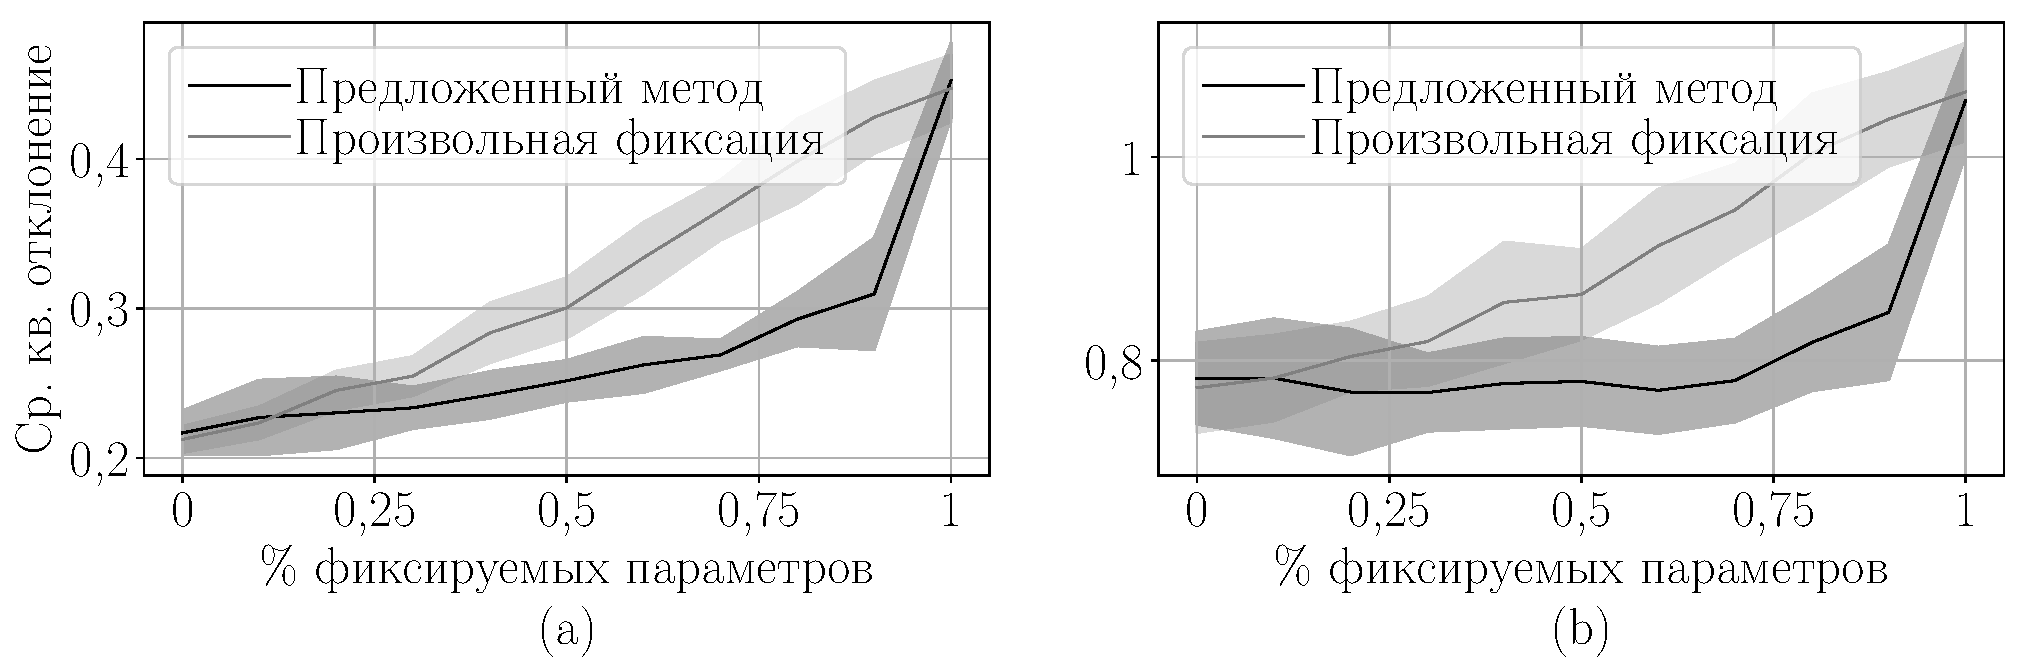
\includegraphics[width=1\textwidth]{results/order/generate_data_neural_loss}
\caption{Зависимость качества модели от числа зафиксированных параметров: a) на обучающей выборке; b) на тестовой выборке}
\label{ch-5:fg:ex:syn3:1}
\end{figure}

\begin{figure}[h!t]\center
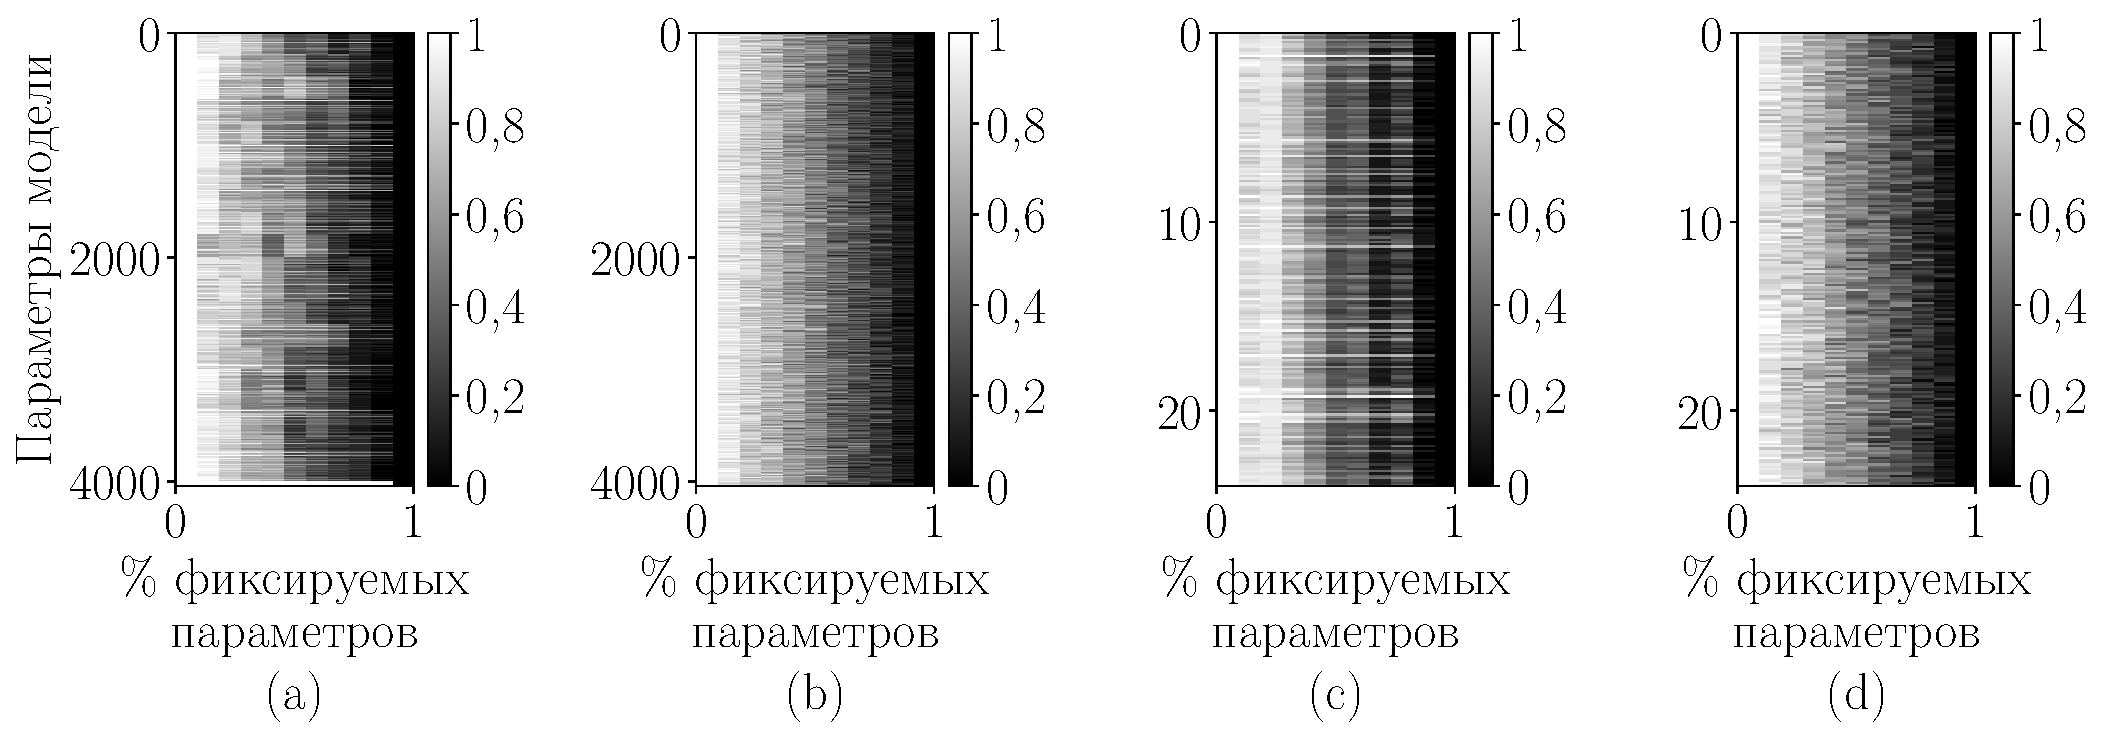
\includegraphics[width=1\textwidth]{results/order/generate_data_neural_matshow}
\caption{Визуализация векторов $\hat{\bm{\alpha}}\bigr(\zeta\bigr)$ в зависимости от числа фиксируемых параметров: a) все параметры модели упорядочены предложенным методом; b) все параметры модели упорядочены произвольным образом; c) часть параметров модели упорядочена предложенным методом; d) часть параметров модели упорядочена произвольным образом}
\label{ch-5:fg:ex:syn3:2}
\end{figure}

Эксперимент проводился на синтетически построенных данных. В качестве модели использовалась двухслойная нейросеть~--- перцептрон.
%На рис. \ref{ch-5:fg:ex:syn3:1} показано, что фиксация параметров в соответствии с предложенным порядком является лучше, чем фиксация параметров произвольным образом, так как функция ошибки растет медленней при фиксации большего процента параметров.
На рис. \ref{ch-5:fg:ex:syn3:1} показаны графики зависимости функции потерь $\mathcal{L}$ от числа фиксируемых параметров. В случае фиксации параметров предложенным методом функция потерь $\mathcal{L}$ растет медленней, чем в случае фиксации параметров произвольным образом.

На рис. \ref{ch-5:fg:ex:syn3:2} показана зависимость векторов $\hat{\bm{\alpha}}\bigr(\zeta\bigr)$ от числа фиксируемых параметров. Каждый столбец соответствует одному вектору $\hat{\bm{\alpha}}\bigr(\zeta\bigr)$. На рис. \ref{ch-5:fg:ex:syn3:2}a, \ref{ch-5:fg:ex:syn3:2}с видно, что $\hat{\bm{\alpha}}\bigr(\zeta\bigr)$ имеет большое число компонент вектора, близких к $1$. Так как $\hat{\bm{\alpha}}\bigr(\zeta\bigr)$ является усреднением вектора с компонентами $0$ или $1$, то предложенный порядок задает некоторый устойчивый порядок на множестве параметров модели. На рис. \ref{ch-5:fg:ex:syn3:2}b, \ref{ch-5:fg:ex:syn3:2}d видно, что в случае произвольной фиксации параметров компоненты вектора $\hat{\bm{\alpha}}\bigr(\zeta\bigr)$ имеют одинаковые значения, следовательно, никакого порядка на множестве параметров нет.

\paragraph{Выборка Boston Housing.}
\begin{figure}[h!t]\center
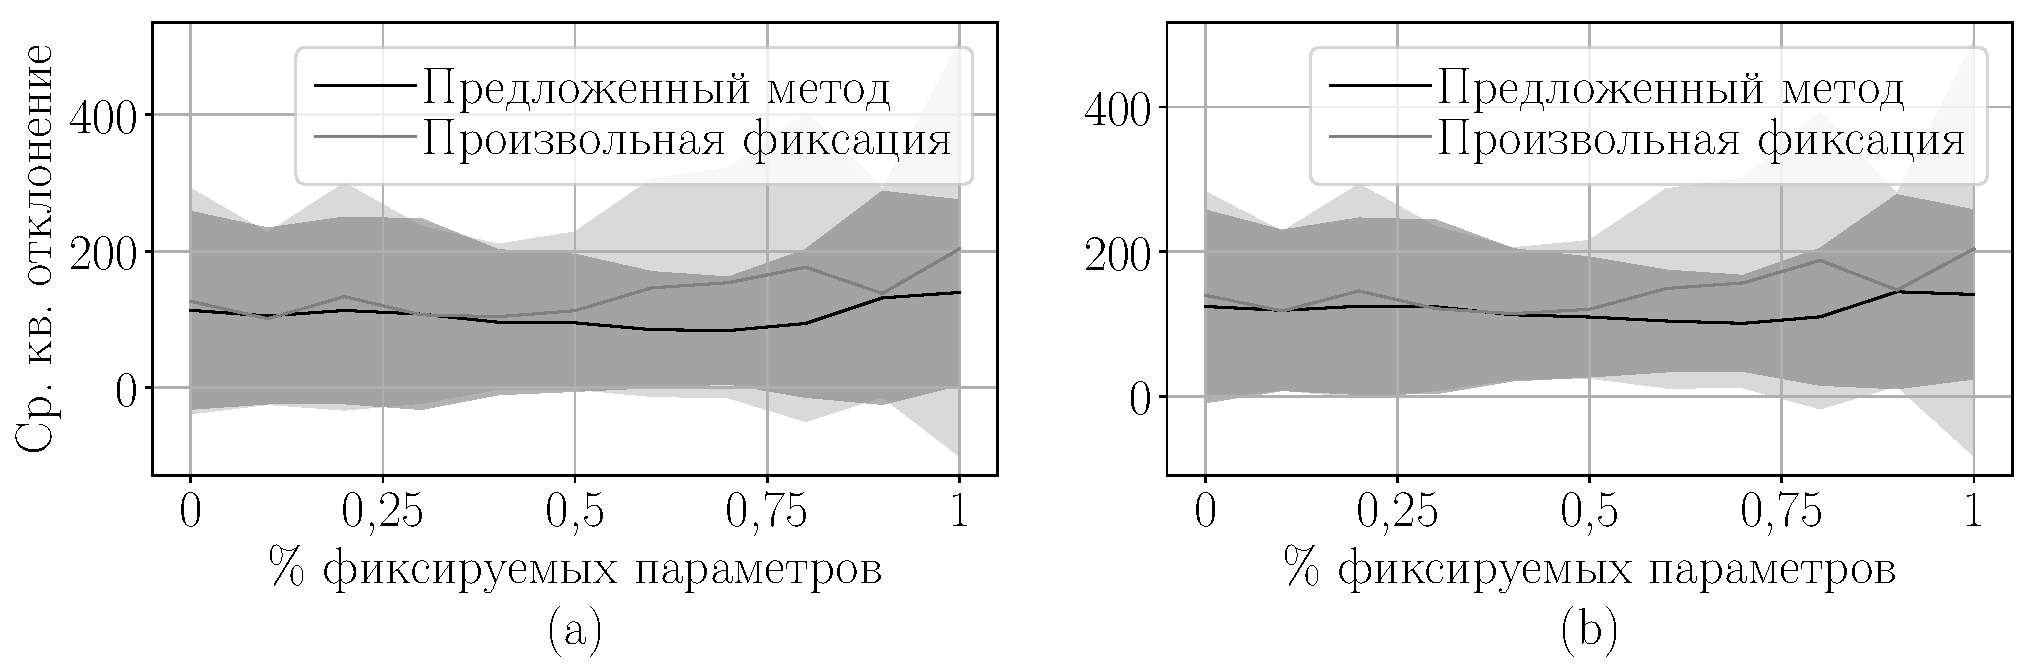
\includegraphics[width=1\textwidth]{results/order/boston_data_loss}
\caption{Зависимость качества модели от числа зафиксированных параметров: a) на обучающей выборке; b) на тестовой выборке}
\label{ch-5:fg:ex:bost:1}
\end{figure}
Эксперимент проводился на реальных данных.
На рис. \ref{ch-5:fg:ex:bost:1} показаны графики зависимости функции потерь $\mathcal{L}$ от числа фиксируемых параметров. В случае фиксации параметров предложенным методом, функция потерь $\mathcal{L}$ растет так же, как и в случае фиксации параметров произвольным образом.
Данный результат следует из того, что нейросеть оказалась избыточно сложной моделью с большим числом параметров. После фиксации значимого числа параметров у модели оставалась большое число параметров для дообучения.

На рис. \ref{ch-5:fg:ex:bost:2} показана зависимость векторов $\hat{\bm{\alpha}}\bigr(\zeta\bigr)$ от числа фиксируемых параметров. На рис. \ref{ch-5:fg:ex:bost:2}a, \ref{ch-5:fg:ex:bost:2}с видно, что $\hat{\bm{\alpha}}\bigr(\zeta\bigr)$ меняется незначительно от запуска к запуску алгоритма. Следовательно, предложенный порядок задает устойчивый к разным запускам порядок на множестве параметров модели. На рис. \ref{ch-5:fg:ex:bost:2}b, \ref{ch-5:fg:ex:bost:2}d видно, что в случае произвольной фиксации параметров вектор $\hat{\bm{\alpha}}\bigr(\zeta\bigr)$ является произвольным и никакого порядка на множестве параметров нет.

\begin{figure}[h!t]\center
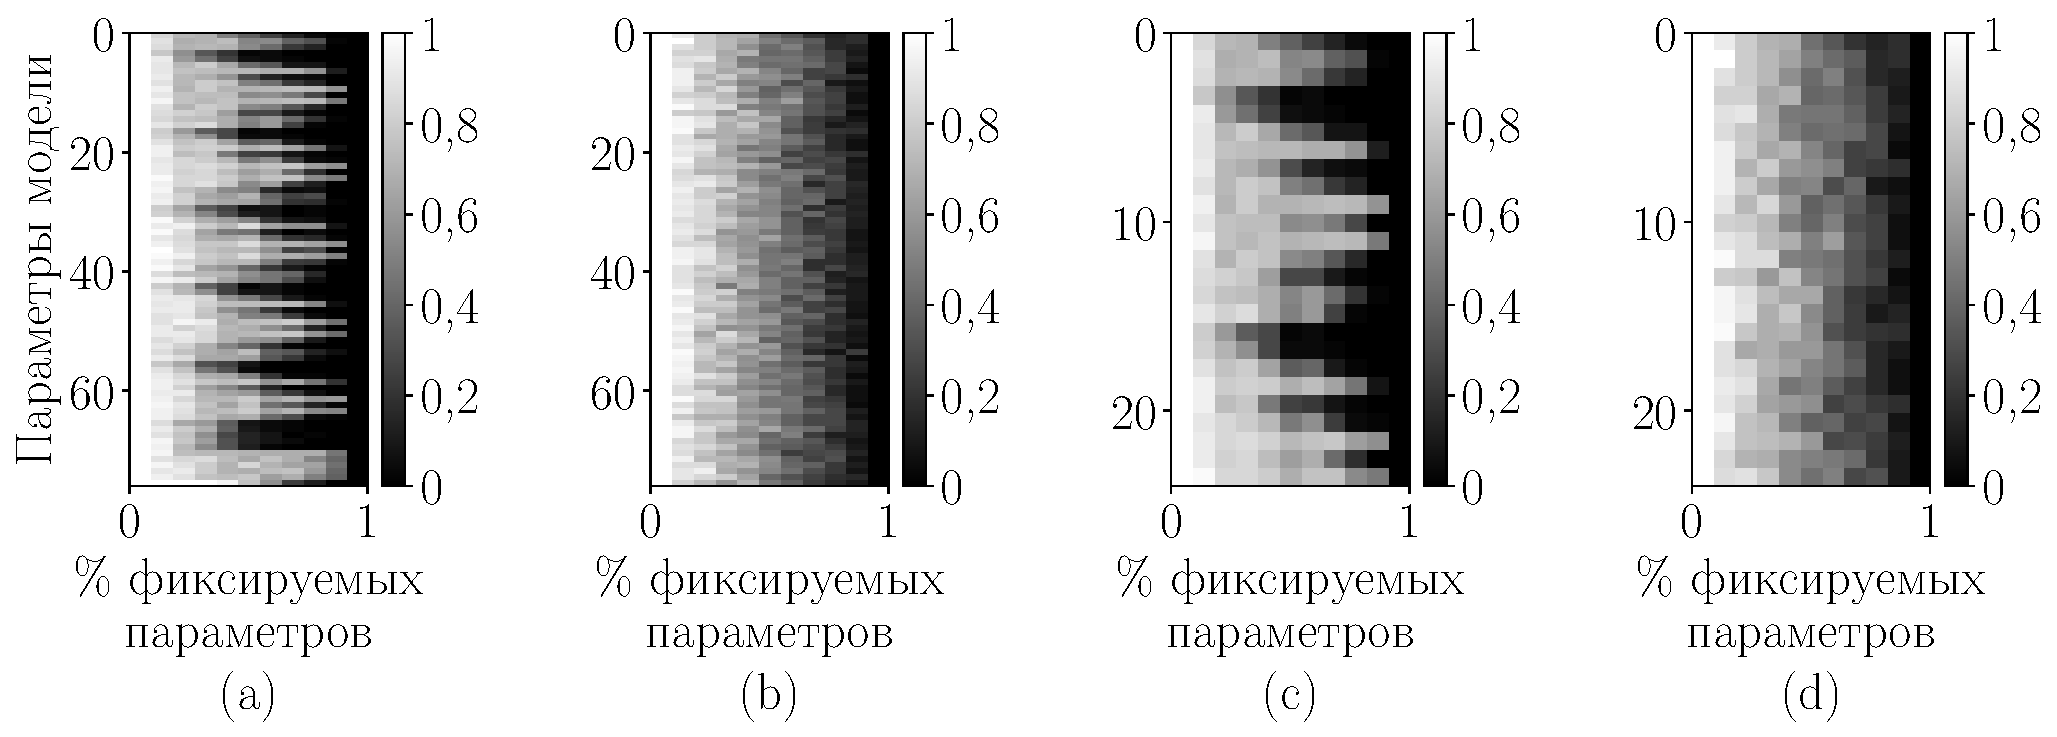
\includegraphics[width=1\textwidth]{results/order/boston_data_matshow}
\caption{Визуализация векторов $\hat{\bm{\alpha}}\bigr(\zeta\bigr)$ в зависимости от числа фиксируемых параметров: a) все параметры модели упорядочены предложенным методом; b) все параметры модели упорядочены произвольным образом; c) часть параметров модели, упорядочена предложенным методом; d) часть параметров модели упорядочена произвольным образом}
\label{ch-5:fg:ex:bost:2}
\end{figure}

\paragraph{Выборка Synthetic 3.}
\begin{figure}[h!t]\center
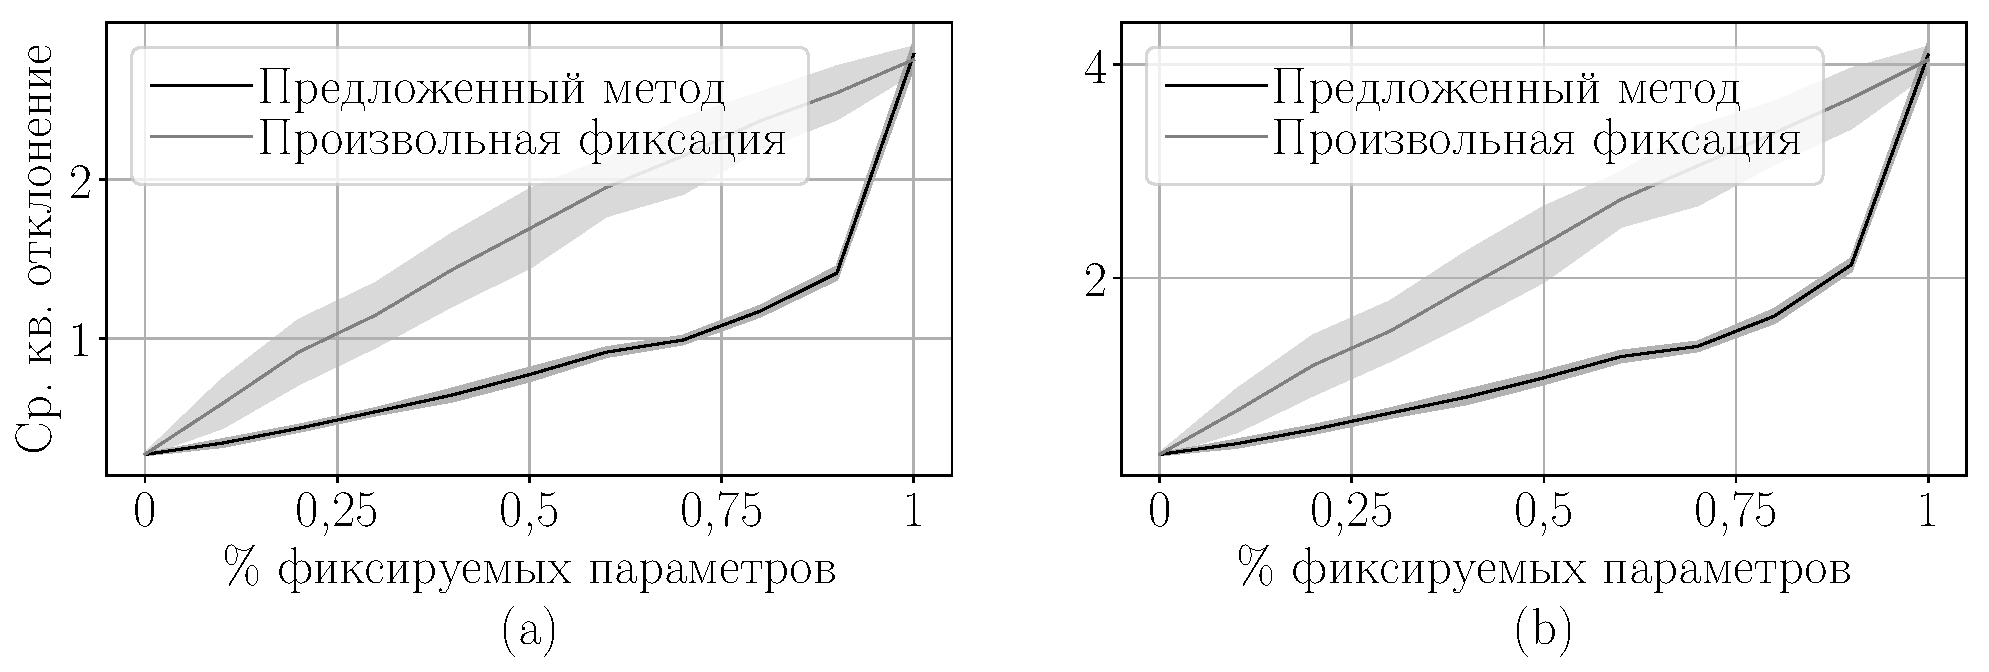
\includegraphics[width=1\textwidth]{results/order/generate_data_linear_loss}
\caption{Зависимость качества модели от числа зафиксированных параметров: a) на обучающей выборке; b) на тестовой выборке}
\label{ch-5:fg:ex:syn1:1}
\end{figure}

\begin{figure}[h!t]\center
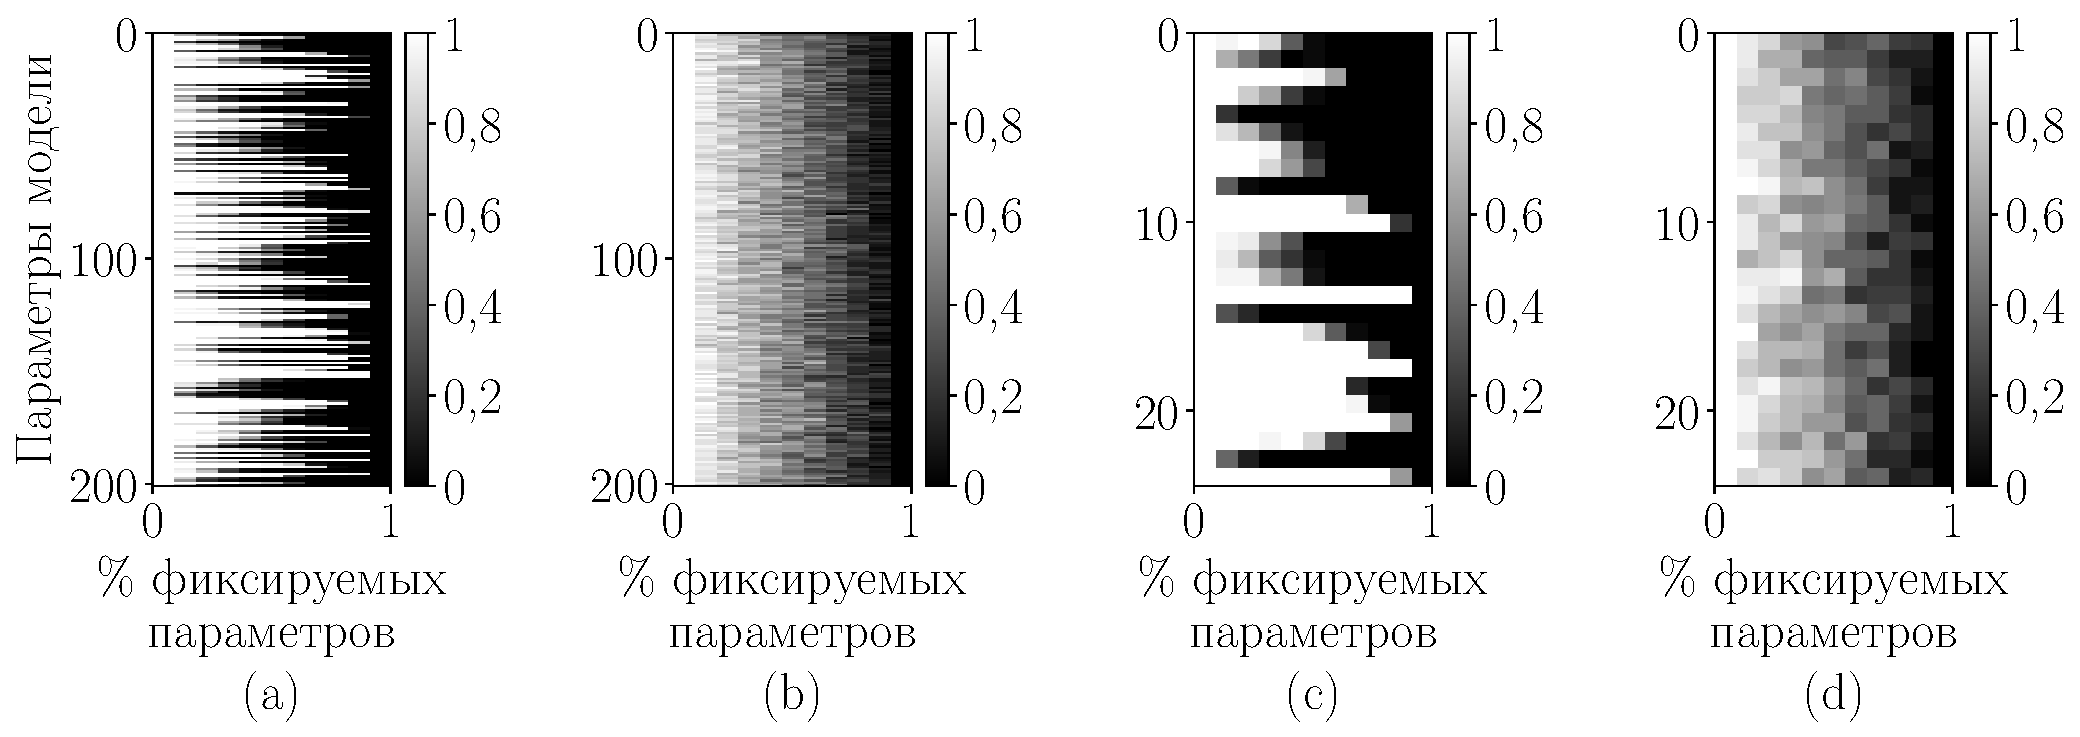
\includegraphics[width=1\textwidth]{results/order/generate_data_linear_matshow}
\caption{Визуализация векторов $\hat{\bm{\alpha}}\bigr(\zeta\bigr)$ в зависимости от числа фиксируемых параметров: a) все параметры модели упорядочены предложенным методом; b) все параметры модели упорядочена произвольным образом; c) часть параметров модели, упорядочены предложенным методом; d) часть параметров модели упорядочена произвольным образом}
\label{ch-5:fg:ex:syn1:2}
\end{figure}

Эксперимент проводился на синтетически построенных данных. В качестве модели использовалась линейная модель регрессии.

На рис. \ref{ch-5:fg:ex:syn1:1} показаны графики зависимости функции потерь $\mathcal{L}$ от числа фиксируемых параметров. В случае фиксации параметров предложенным методом функция потерь $\mathcal{L}$ растет значительно медленней в сравнении со случаем фиксации параметров произвольным образом. Дисперсия функции ошибки также значительно меньше в случае фиксации параметров предложенным методом.

На рис. \ref{ch-5:fg:ex:syn1:2} показано, что вектора $\hat{\bm{\alpha}}\bigr(\zeta\bigr)$ не меняется от запуска к запуску. Так как данная модель линейная, то порядок на параметрах модели индуцирует некоторый порядок на множестве признаков.

\paragraph{Выборка MNIST.}

\begin{figure}[h!t]\center
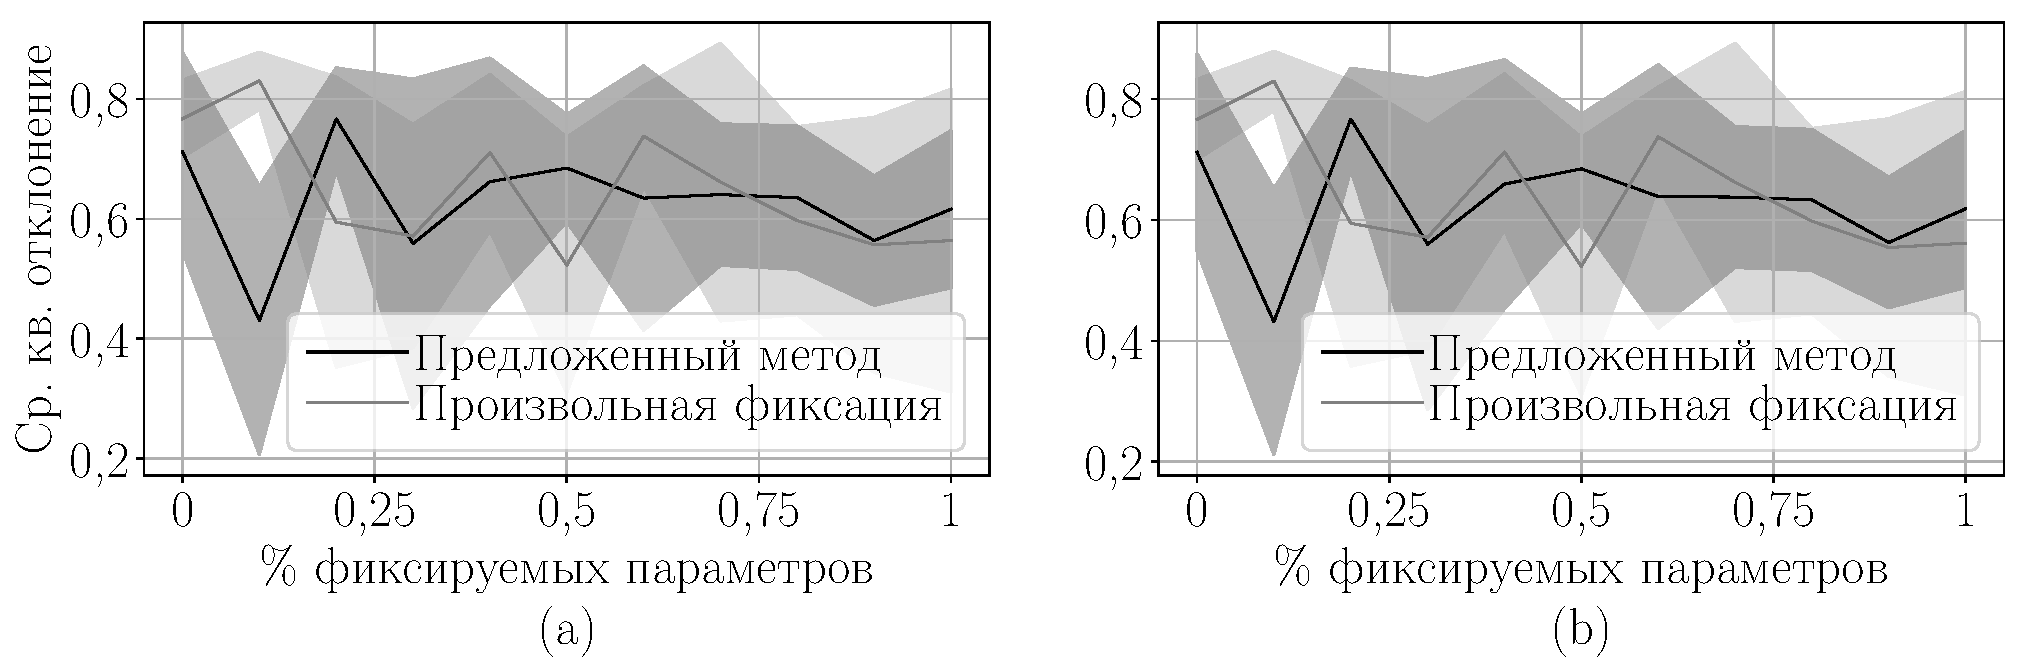
\includegraphics[width=1\textwidth]{results/order/mnist_data_loss}
\caption{Зависимость качества модели от числа зафиксированных параметров: a) на обучающей выборке; b) на тестовой выборке}
\label{ch-5:fg:ex:mnist:1}
\end{figure}

\begin{figure}[h!t]\center
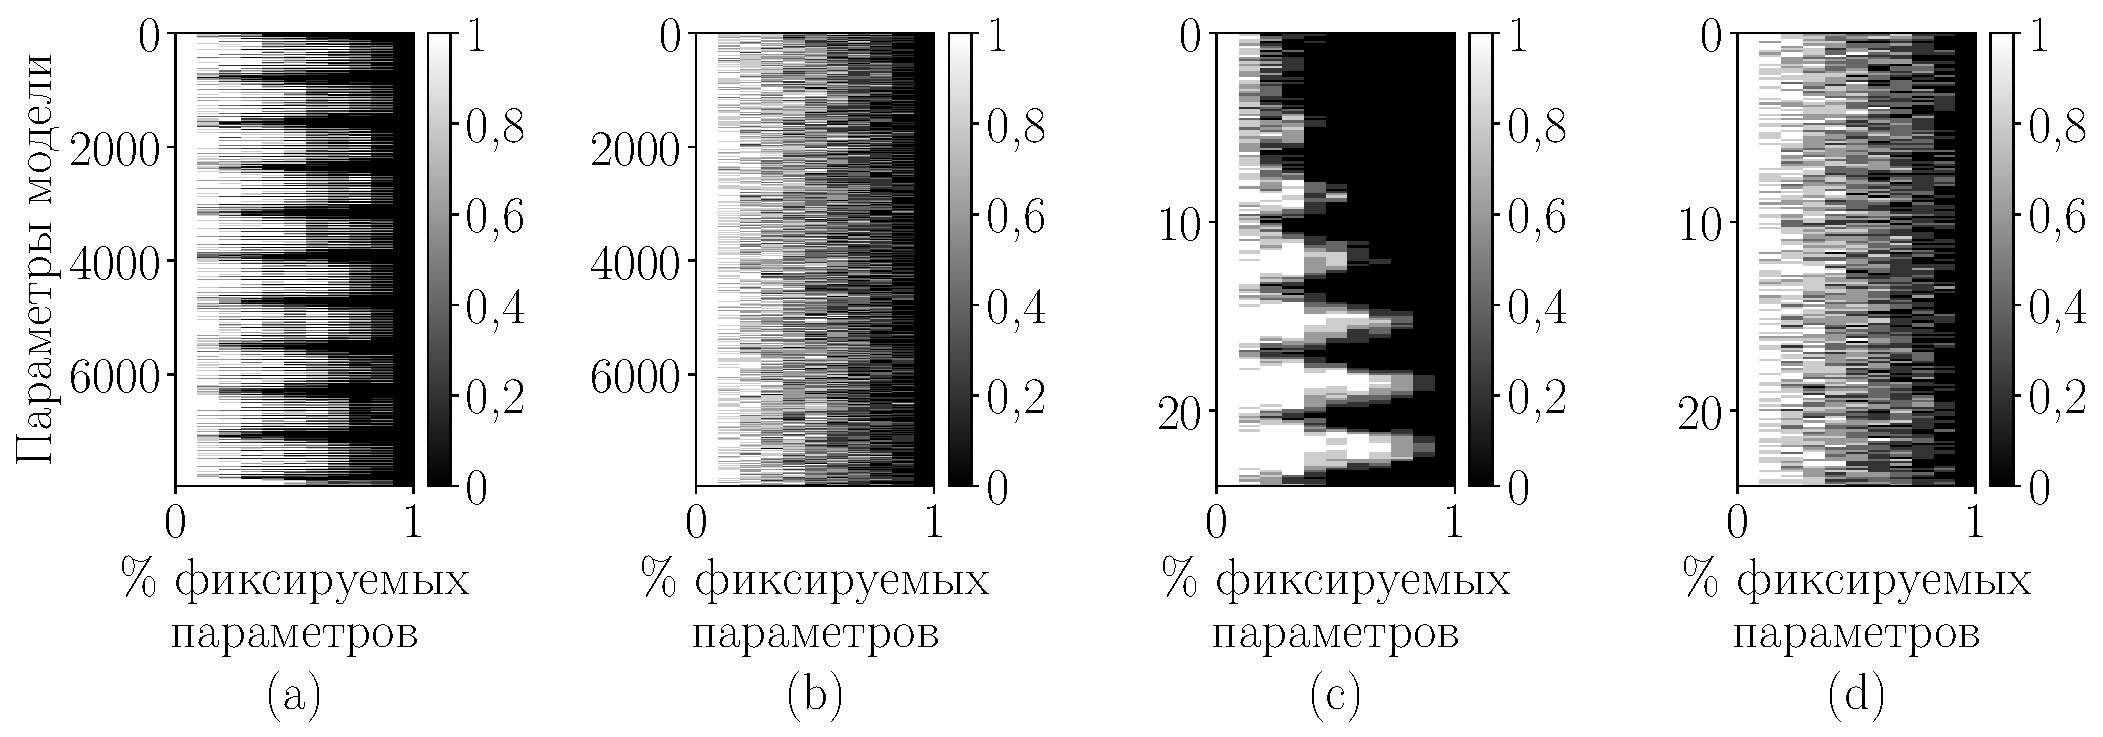
\includegraphics[width=1\textwidth]{results/order/mnist_data_matshow}
\caption{Визуализация векторов $\hat{\bm{\alpha}}\bigr(\zeta\bigr)$ в зависимости от числа фиксируемых параметров: a) все параметры модели упорядочены предложенным методом; b) все параметры модели упорядочены произвольным образом; c) часть параметров модели упорядочена предложенным методом; d) часть параметров модели упорядочена произвольным образом}
\label{ch-5:fg:ex:mnist:2}
\end{figure}

В эксперименте рассматривался двухслойный перцептрон для классификации изображений. В качестве входных данных рассматривались изображения размера $28\times28$, на которых изображены цифры. 

На рис. \ref{ch-5:fg:ex:mnist:1} показано, что графики функции ошибки похожи в случае фиксации параметров параметров предложенным методом и в случае произвольной фиксации. Данный результат есть следствие того факта, что нейросеть является заведомо переусложненной моделью с большим числом параметров. После фиксации большого числа параметров у нейросети все еще остается значимое число параметров модели для дообучения.

На рис. \ref{ch-5:fg:ex:mnist:2} показано, что в случае модели со значимым числом оптимизационных параметров,предложенный метод упорядочения параметров устойчив от запуску к запуску.

